\documentclass[long, final]{jobim2017}
% Available options are:
% - showframe 
% - draft
% - final [default]

\usepackage[utf8]{inputenc}

% WARNING: already loaded packages:
% - hyperref
% - times
% - color
% - xspace
% - graphicx
% - fancyhdr
% - fancybox
% - indentfirst
% - geometry
% - babel (options english,francais) :
%   choose the language with \selectlanguage{<language>}


\pagestyle{empty}
\addtolength{\parskip}{0.4\baselineskip}

%% Title of the paper (required)
\title{Data updates on Norine, the reference Non-Ribosomal Peptide knowledge base}

%% List of authors (separated by the macro \and).
%% Authors can be followed by \inst{<n>} macro.
%% The <n> parameter of the \inst macro should correspond to the <n>th institution
%% (see macro \institute below).
\author{Yoann \textsc{Dufresne}\inst{1} \and Juraj \textsc{Michalik}\inst{1} \and Areski \textsc{Flissi}\inst{1}
\and Valerie \textsc{Leclère}\inst{1, 2} \and Maude \textsc{Pupin}\inst{1}}

%% List of institutions (separated by the macro \and).
\institute{
 Équipe Bonsai, Univ. Lille, CNRS, Centrale Lille, UMR 9189 - CRIStAL - Centre de Recherche
en Informatique Signal et Automatique de Lille, F-59000 Lille, France
 \and
 Équipe ProBioGEM, Univ. Lille, INRA, ISA, Univ. Artois, Univ. Littoral Côte d’Opale, EA 7394 -
ICV - Institut Charles Viollette, F-59000 Lille, France
}

% email of the corresponding author
\corresponding{yoann.dufresne0@gmail.com}





%% Abstract of the paper (required).
\abstract{%
Norine is the unique knowledge-base dedicated to non-ribosomal peptides. Those peptides have the particularities of containing monomers other than the 20 amino acids and having complex structures with cycles and branches. Since 2006, Norine is filled in manually by extraction of annotations from scientific literature and contains 1186 peptides. But, the annotation process is time consuming and fastidious. One of the bottlenecks is the determination of the monomeric structure because it is rarely given in articles. The development of the software smiles2monomers (s2m) that infers a monomeric structure from an atomic one has opened new opportunities for Norine completion and curation. Firstly, s2m has detected few incoherences between stored structures. We are currently curating those structures. Secondly, we open Norine to crowdsourcing and provide s2m as a tool to help the scientists entering accurate structures. Finally, we develop scripts to automatically extract peptides and their annotations from other databases. With those strategies, we will be able to keep Norine up-to-date by multiplying data sources and to improve annotation quality by making structure validation.
}




%% List of keywords of the paper (required).
\keywords{Norine database, Non-Ribosomal Peptides, Update, Data curation}

\begin{document}

 % Si vous écrivez en français, commentez la ligne suivante
\selectlanguage{english}
 % Si vous écrivez en francais, décommentez la ligne suivante...
 % \selectlanguage{francais}

   \maketitle





\section{Introduction}

Norine, first released in 2006~\cite{caboche_norine:_2008}, remains the unique platform dedicated to computational analysis of non-ribosomal peptides (NRPs). The NRPs have increased in popularity in recent years because they harbour diverse interesting biological activities.
Indeed, they are produced by micro-organisms, bacteria and fungi, to colonise and survive in various environments.
Among others, NRPs can act as antibiotics (penicillin -NOR00006-, daptomycin -NOR00001- or vancomycin -NOR00681-), siderophores (pyoverdins -NOR00160 to 206, NOR00903 to 912- or vibriobactin -NOR00250-), surfactants or protease inhibitors.
In addition to their primary activity, some NRPs are also successfully prescribed for treating cancers (actinomycin D -NOR00228-) or reducing transplant rejection (cyclosporin A -NOR00033-).
Beyond the pharmacology, NRPs promise other advantageous applications such as biocontrol of plant diseases, bioremediation of areas contaminated with toxic metals and/or non-biodegradable organic compounds.
These metabolites are produced by a specific biosynthetic pathway.
In few words, huge enzymes called NRP synthetases select specific amino acids, variant amino acids, lipids (and many other) and assemble them.

 \begin{figure}
   \begin{center}
     % if you have pdflatex installed, you can use pdf files as graphics
     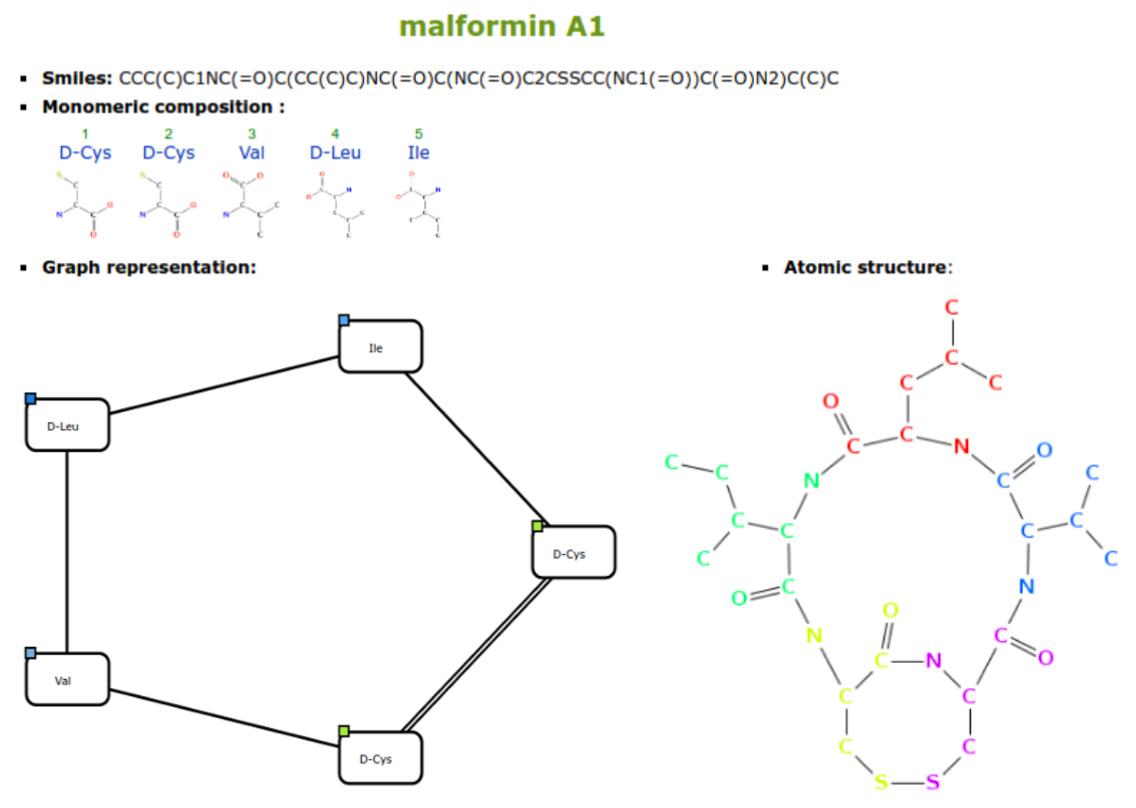
\includegraphics[width=400px]{figs/malformin_A1.png}
     % On the other hand, you must use eps files
     % \includegraphics[height=4cm,width=6cm]{figs/fig1.eps}
   \end{center}
   \caption{Structure representations of the malformin A1 in the Norine database.}
   \label{fig:malformin}
 \end{figure}


The Norine database is the reference NRP knowledge base, containing more than 1200 peptides composed of almost 530 different monomers (different building blocks including amino acids).
In the database, each NRP referenced have a dedicated web page with various informations about their provenance, their composition and their biological activities.
The most important information is their monomeric structure/composition (see figure \ref{fig:malformin}, on the left).
The monomeric representation, that we also called the biological structure, correspond to the nearest representation of the NRP assembly process.
In this representation, each node correspond to a monomer that have been included during the synthesis.
The other representation (figure \ref{fig:malformin}, on the right), is the atomic representation, obtained by reconstruction after a mass spectrum analysis.
The knowledge of the monomeric representation is the most important information about a peptide because it is needed to fully understand the synthesis pathway.
It as also been proved~\cite{abdo_new_2012} that, in most cases, the activity of the molecule can be predicted from this single representation.

Since 2016, the Norine database is open to crowdsourcing~\cite{flissi_norine_2016}.
External users can submit new peptides to improve the data quantity of the database.
A complete procedure of submission and reviewing have been set up to guaranty the quality of the new annotation.
Nevertheless, we know that many NRP discovered are not present in the Norine database and this process is not allowing a massive addition of data.
It is also not allowing the correction of wrong data that has been entered before the set up.

In the next parts of this article we will have a quick overview of the current work on data curation and database filling.


\section{Improving the data quality}

In the Bonsai group, we developed a tool called smiles2monomers (s2m)~\cite{dufresne_smiles2monomers:_2015} that automatically creates annotations of NRP.
From a SMILES~\cite{weininger_smiles_1988} (a textual atomic representation of a molecule), s2m infer the monomeric structure of the NRP.
On one side, as we said in the introduction, the most useful information is the monomeric structure of NRP.
On the other side, almost every NRP are characterised by mass spectrum experiments, so we often only know their atomic structure.
So, s2m is a very powerful tool for the NRP community, making the link between both annotations.

 \begin{figure}
   \begin{center}
     % if you have pdflatex installed, you can use pdf files as graphics
     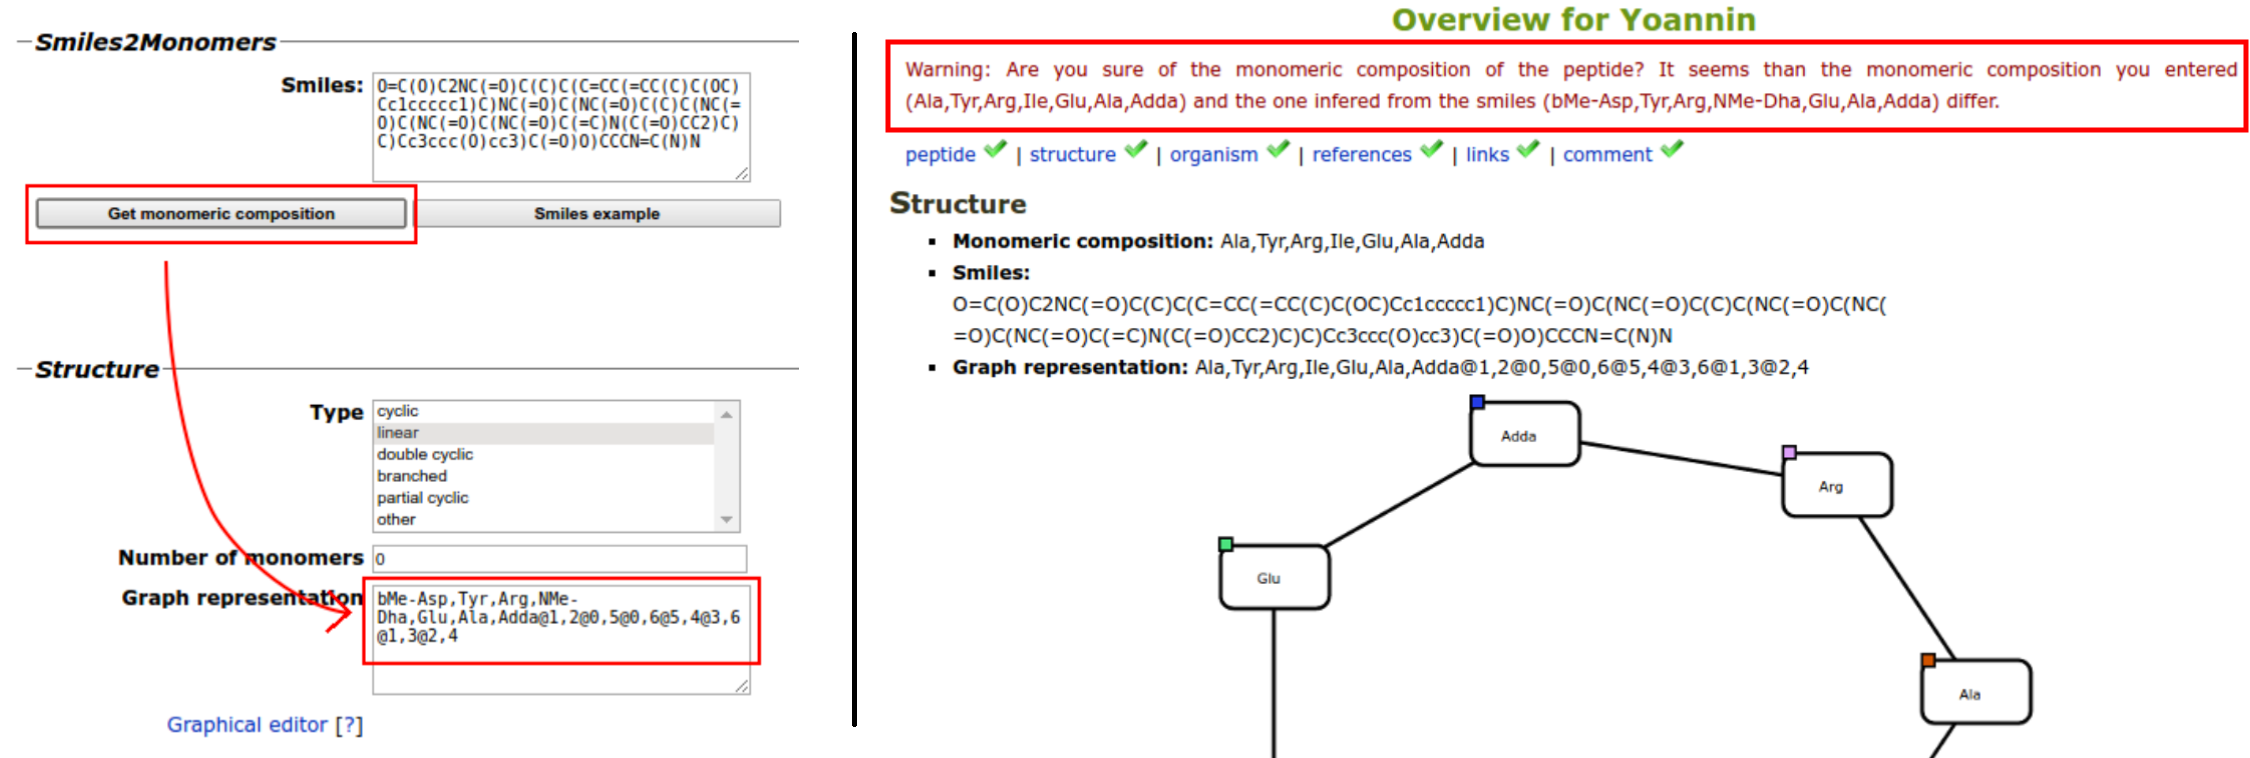
\includegraphics[width=400px]{figs/warnings.png}
     % On the other hand, you must use eps files
     % \includegraphics[height=4cm,width=6cm]{figs/fig1.eps}
   \end{center}
   \caption{Quality controls in the MyNorine software.}
   \label{fig:warnings}
 \end{figure}

In the Norine database, a significant amount of NRP entries (around 30\%) are filled with both atomic and monomeric structures.
We used s2m on the atomic structures to verify the integrity of the data and we found a few errors (50 NRPs with a wrong atomic or monomeric structure).
To avoid the insertion of new errors, we included the s2m software in the crowdsourcing tool MyNorine.
When a user wants to add a new compound s2m is used during two validation steps.
Firstly, when the user fills the SMILES area, myNorine can automatically creates the monomeric structure (see figure \ref{fig:warnings}, on the left).
Secondly, if the user did not explicitly generate the monomeric structure, s2m runs in background to compare the result with the manually entered structure.
If the automatic and manual annotations are not equivalent, the MyNorine tool raises a warning to the user (see figure \ref{fig:warnings}, on the right)


\section{Improving data quantity}

Norine was created in 2006 and updated until 2016 by a small group of people.
Many NRPs published were added to the database but we know that a lot of other molecules, for many different reasons, has never been published, even if they are fully characterised.
Aiming the goal of adding all theses NRPs to Norine, we opened the database to crowdsourcing.
Since this opening, a multitude of NRP have been added but many NRPs not present in Norine are present in other specialised and unspecialised databases of molecules.

We identified 3 main databases that can be sources of new NRPs for Norine.
The first one is the Minimum Information about a Biosynthetic Gene cluster (MIBiG) database~\cite{_mibig:_????}.
This database stores information about gene clusters of secondary metabolites, including NRPs.
The second one is the Biologically Interesting Molecule Reference Dictionary (BIRD)~\cite{berman_announcing_2003}.
This database references external resources about "interesting" molecules and we know that some of them are NRPs.
The last database used as resource is StreptomeDB~\cite{lucas_streptomedb:_2013}, the database that reference the molecules produced by bacteria in the \textit{Streptomyces} genus.
These bacteria are known as producers of NRP and that's why we explored this database.
Until now, the Norine database is well known for the quality of its manual annotations.
So, we did not want to add wrong informations from an automatic filling of the database and that's why we created a strict validation pipeline for the potential new entries.
After the filtering process that I will describe in the next paragraph, we found 472 NRPs unreferenced in Norine: 235 from MIBiG, 162 from BIRD and 75 from StreptomeDB.

 \begin{figure}
   \begin{center}
     % if you have pdflatex installed, you can use pdf files as graphics
     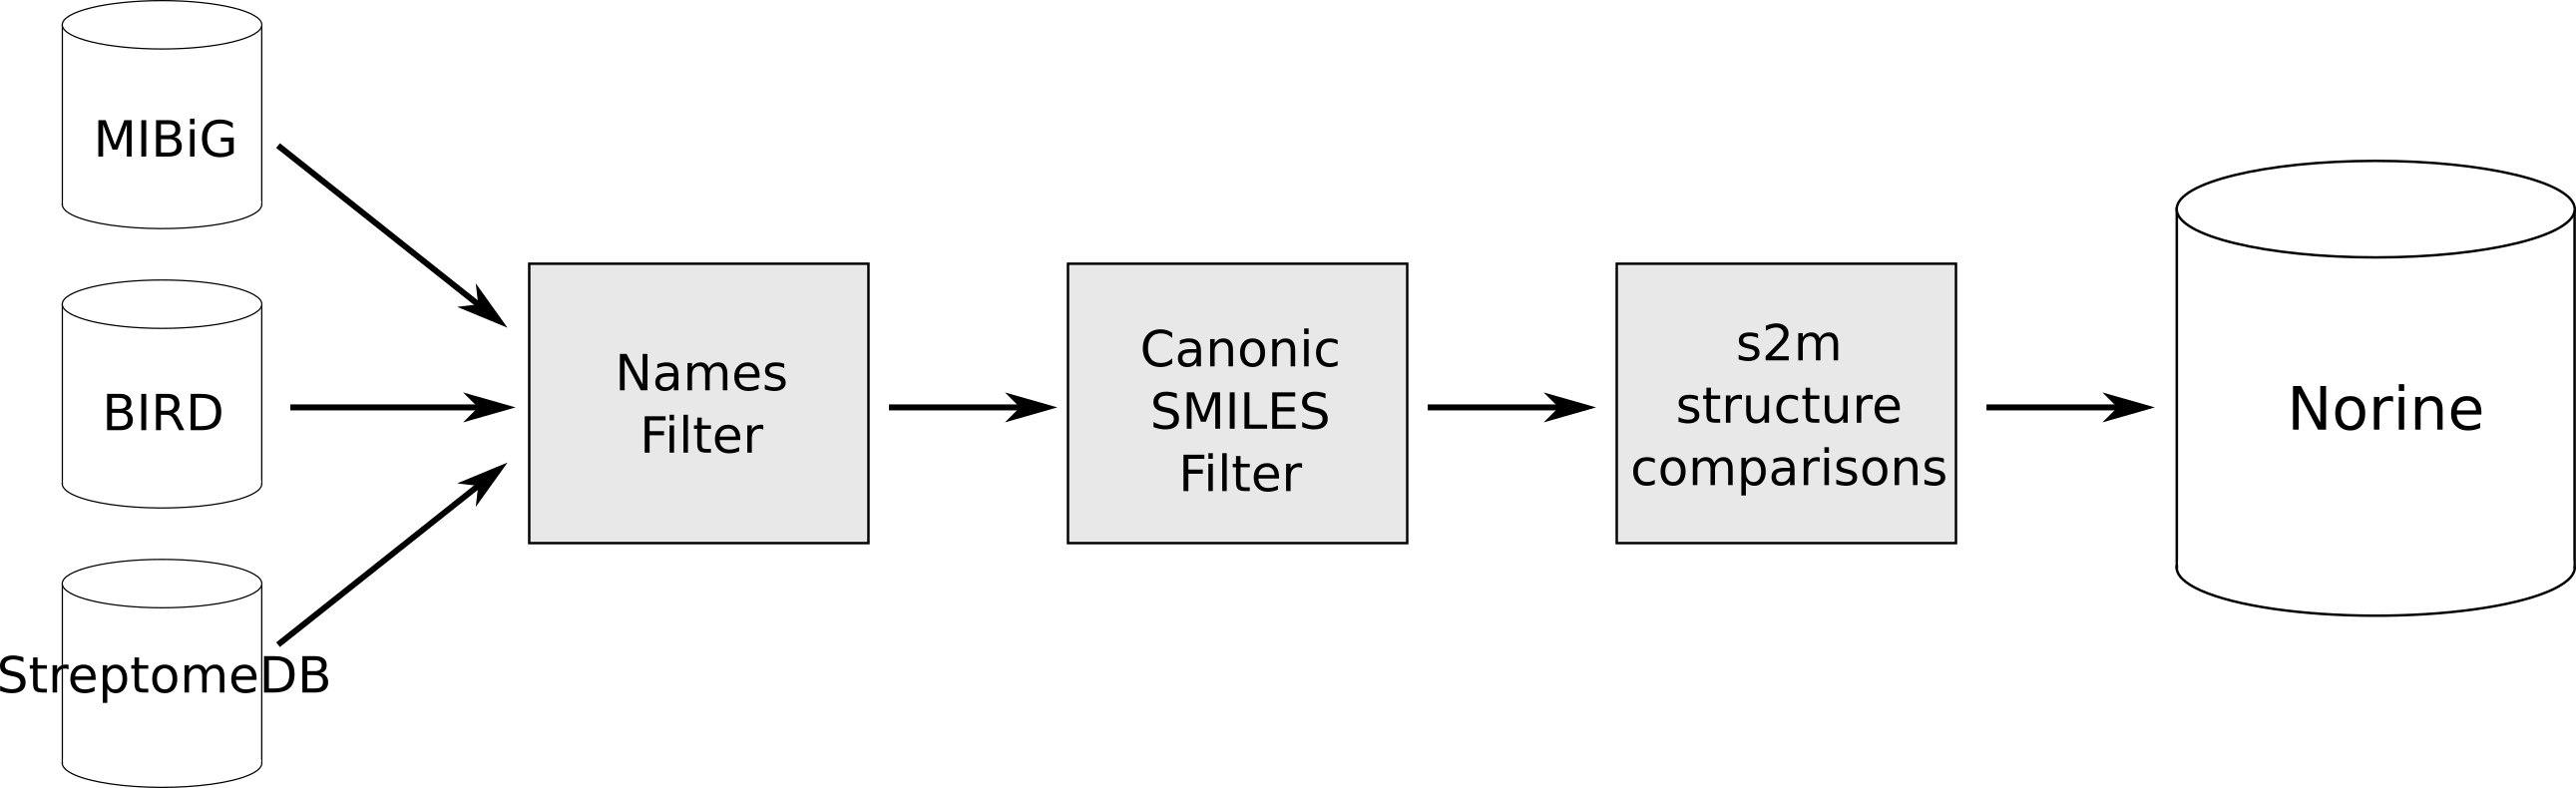
\includegraphics[width=400px]{figs/filters.png}
     % On the other hand, you must use eps files
     % \includegraphics[height=4cm,width=6cm]{figs/fig1.eps}
   \end{center}
   \caption{Automatic filing quality control.}
   \label{fig:quality}
 \end{figure}

To automatically include new entries, we created a pipeline of filters based on name, SMILES and structure comparisons (see figure \ref{fig:quality}).
Before all the filtering tasks, we only extract molecules that are already annotated as NRP in the databases.
First, we filter by names and known synonyms to avoid duplicated entries (fast and easy task).
Then, we try to avoid duplicates using a string comparison of SMILES.
For this task, we use the CDK library~\cite{steinbeck_chemistry_2003} to get a canonical SMILES from each candidate entry (multiple SMILES can represent a single molecule; a canonical SMILES is always the same for one molecule).
Those canonical SMILES are used to compare the candidate entry to all the SMILES already present in the database (the canonization is time consuming but the string comparison is fast).
Finally, for the molecules not filtered, we compute and compare the monomeric graph with monomeric graphs stored in Norine.
For this task, we use s2m to generate the monomeric graphs and a simple algorithm of graph isomorphism to compare the graph against the database (the most time consuming task).

After the execution of these scripts, the database was filled with 472 new peptides and their annotations.
Those data represent an increase of 30\% of the entries in the Norine database for a new total of 1658 annotated NRPs.
For the data that where already present in Norine, we are currently looking at the similarities and differences between our annotations and the ones of the other databases to select the best combination of both.


\section{Conclusion and perspectives}

In this article we presented an update of the data from the knowledge base Norine.
Using tools like smiles2monomers, we detected a few errors in the annotations.
We corrected them and created safeguards to avoid errors in future user submissions.
In a second time, we used several tools to retrieve and filter many possible new NRP entries in the database.
The work on automatic filing scripts led us to a data increase of 30\% for a new total of 1658 peptides in Norine.
So, in the coming release of Norine we strongly improve the data quantity and quality available for all.

We also noticed that many data remain absent from the database.
For example, we noticed that some entries in the PubChem database are undiscovered NRP (not associated to NRP keyword).
We soon will be able to screen the entire PubChem database and automatically relate peptides to proof of their non-ribosomal synthesis.



 \bibliography{jobim_proceedings}
 
\end{document}

